%% *************************************************************************
%%
%% This is an RIT Space Exploration Standard defining guidelines for content
%% and formatting of project design documents.
%%
%% This document uses IEEEtran.cls, the official IEEE LaTeX class
%% for authors of the Institute of Electrical and Electronics Engineers
%% (IEEE) Transactions journals and conferences.
%%
%% *************************************************************************

%% *************************************************************************
% LaTeX REFERENCES
% ----------------
%   Intro to LaTeX: http://www.rpi.edu/dept/arc/docs/latex/latex-intro.pdf
%   Comprehensive LaTeX symbol list: http://tug.ctan.org/info/symbols/comprehensive/symbols-a4.pdf
%% *************************************************************************

% tell \LaTeX what kind of formatting to use
\documentclass[conference]{IEEEtran} % http://www.ctan.org/pkg/ieeetran
% enable placeholder text generator
\usepackage{blindtext}
% enable toolbox for embedding figures and pictures
\usepackage{graphicx}
% enable package for adding a list of variables and constants at the beginning, aka "nomenclature"
\usepackage{nomencl}
% enable package for easily formatting units
\usepackage{siunitx}
% enable package for cross-referencing figures, sections, references etc.
% how to use hyperref: http://www2.washjeff.edu/users/rhigginbottom/latex/resources/lecture09.pdf
\usepackage{hyperref}
% change text encoding to make it more crisp
\usepackage[T1]{fontenc}
% enable conditionals for help text
\usepackage{etoolbox}

% initialize nomenclature package
\makenomenclature{}

% set title. choose something as descriptive and precise as possible. Descriptive > sounding cool. remember this!
\title{RIT Space Exploration Participation in the Intercollegiate Rocket Engineering Competition}


\author{
  % List the authors of the design document. The Champion should go first.
  % The \$~\$ markers tell \LaTeX{} to treat the text inside to be treated as a math expression. This way you can use operators like \textcaret{} to place characters as superscripts.
  % Some \LaTeX{} templates handle the author block in different ways. For example, the \href{http://www.worldscientific.com/worldscinet/jai}{Journal of Astronomical Instrumentation} requires the authors' addresses and emails to be included as well.
  % The \textbackslash{}thanks command puts the contents inside those brackets in a footnote at the bottom of the first page. Technically speaking, \textbackslash{}thanks is just a specially formatted footnote.
  % IEEE also has a ``long form'' author block for many authors. Check here for more information:
  % \url{https://tex.stackexchange.com/questions/156523/multiple-authors-with-common-affiliations-in-ieeetran-conference-template}
  % Read here for a more advanced options to modifying footnotes in the author block:  \url{http://tex.stackexchange.com/questions/826/symbols-instead-of-numbers-as-footnote-markers}
  %   Here, we use the IEEE long-form author block.
  \IEEEauthorblockN{% This block is for author Names.
    Daniel~Mitchell  %the number in the bracket is a reference number to identify this footnote. \LaTeX will figure out what symbol to put there.
  }
  \IEEEauthorblockA{% This block is for the author Affiliations, aka department and university
    RIT Space Exploration, Rochester Institute of Technology \\ %\\ starts a new line
    Rochester, N.Y. \\
    Email: ddm9599@rit.edu
  }
  %%   Below, we use the short-form author block and basically hack it to suit our needs.
  % Philip~Linden$^{*\dagger}$%
  %   \thanks{$^{*}$Project Champion}%
  %   \thanks{$^{\dagger}$BS/MEng '17, Mechanical Engineering},
  % Austin~Bodzas$^{\ddagger}$%
  %   \thanks{$^{\ddagger}$BS '19, Computer Science},
  % Drew~Walters$^{\S}$%
  %   \thanks{$^{\S}$BS '18, Mechanical Engineering Technology},
  % T.J.~Tarazevits$^{**}$%
  %   \thanks{$^{**}$BS '19, Game Design \& Development}%

  %%   If there are many authors, consider using symbolic, numeric (aka arabic),  alphabet footnotes or a combination thereof.
  %% the recommended order for symbolic footnotes is
  %%   (1) asterisk        *   *
  %%   (2) dagger          †   \dagger
  %%   (3) double dagger   ‡   \ddagger
  %%   (4) section symbol  §   \S
  %%   et cetera. For higher counts, use 2x symbols (1)-(4) (i.e. (5) two asterisks **). Keep cycling through (1)-(4) using 3x, 4x, and so on.
  %%   Note that these symbol codes work in math mode and text mode.
  %%   There are ways to make LaTeX do this for you, but it is more advanced and not entirely necessary, especially for short author lists. Not worth the hassle, in my opinion.
}
% page header for pages other than cover page
\markboth{IREC Project Design Document}%
{Mitchell \MakeLowercase{\textit{et al.}}: RIT Space Exploration}

% Initial setup is over, start building the document itself
\begin{document}
\maketitle%
% correct bad hyphenation here, separated by spaces
\hyphenation{explor-ation}

\begin{abstract}
 The Intercollegiate Rocket Engineering Competition is a well-known competition among those interested in amateur rocket engineering as well as those
 who do so professionally. With over 110 participating teams, it is the world's largest university rocket competition. Every year, more and more
 organizations are getting involved such as the Space Dynamics Laboratory who sponsors the SDL Payload Challenge. By cooperatively partnering with
 RIT Launch Initiative and their rocket-manufacturing experience, SPEX has an incredible opportunity to display engineering design proficiency and
 an extreme passion for space by creating a custom scientific payload to integrate with Launch Initiative's custom rocket.


      % The abstract is a brief summary of the design document. Typically it includes the purpose of the design document, key goals or objectives, and justifications.
      % Be sure not to confuse the abstract with the introduction.
      % It is easiest to write the abstract after the rest of the paper has been written.
      % That way you can choose key information from the sections that you've already completed and string them together in the abstract.
      % Consider the abstract to be your elevator pitch to anyone reading this design document.
      % What are they reading?
      % What is the goal?
      % Why is it worth my time?
      % The abstract is what will show up in Google results and other search engines, and what people will read when they are deciding what is worth their time and brain power.
\end{abstract}

\label{sec:nomenclature}
\newcommand{\nomunit}[1]{%
\renewcommand{\nomentryend}{\hspace*{\fill}#1}}
\renewcommand{\nompreamble}{
    % If you include mathematical expressions or express variables in the design document, list them with their corresponding definitions here as a list.
    % The two lines below make it look nice when defining units/values to constants.

    % Note that math terms and non-math terms are separated and alphabetized, regardless of the order in which they are defined. (Recall terms \$like this\$ are in the math environment)
    % Read more about advanced nomenclature formatting here:\\
    % \url{https://www.sharelatex.com/learn/Nomenclatures}
  }
\nomenclature{LI}{Launch Initiative}
\nomenclature{RIT}{Rochester Institute of Technology}
\nomenclature{PDD}{Project Design Document}
\nomenclature{IREC}{Intercollegiate Rocket Engineering Competition}
\nomenclature{SPEX}{RIT Space Exploration}
\nomenclature{SDL}{Space Dynamics Laboratory}
\nomenclature{ESRA}{Experimental Sounding Rocket Association}
% Below are examples of using nomenclature for math symbols and constants or units
% \nomenclature{$\dot{m}$}{Mass flow rate
%   \nomunit{\,\si{\kilo\gram\per\second}}}
% \nomenclature{$c$}{Speed of light
%  \nomunit{\,\SI{2.9979e8}{\meter\per\second}}}
\printnomenclature{}


% HELPFUL HINT: If you get the warning ``Command terminated with space.'' when using a \command try placing ``%'' or ``{}'' immediately following the command.

% The sections included here are required. Additional sections and subsections may be added as necessary.
\section{Introduction}
\label{sec:Introduction}
  % The introduction is a place to give background and context before diving into the subject matter.
  % Establish context for the work you are about to propose and the main ideas of the proposition itself.

\IEEEPARstart{T}{he} Intercollegiate Rocket Engineering Competition is an annual event hosted by ESRA for student rocketry teams from across the USA and around the world.
Beginning in 2017, IREC became the flagship activity of a new event called the Spaceport America Cup which is held annually in the desert of Las Cruces, New Mexico.
The competing rockets are typically seen with a diameter of 4 to 8 inches, a length of anywhere from 8 to 20 feet, and will travel to an altitude of either 10,000 or 30,000
feet depending on whether the competing team opts to enroll into the basic or advanced category. The Space Dynamics Laboratory sponsors a separate competition at the
Spaceport America Cup called the SDL Payload Challenge where scientific payloads integrated into the IREC rockets are judged based on criteria such as scientific relevance and technical execution.

The RIT Space Exploration team is a student-faculty research organization dedicated to giving students the opportunity to gain hands-on experience by working with space systems.
By cooperating with Launch Initiative, SPEX would like to enter IREC in the basic category. LI will provide the rocket body and the rocket engine while SPEX will focus on the
integrated scientific payload with the intent of competing in the SDL payload challenge.

\section{Primary Objective}
\label{sec:Primary Objective}
  % At the end of the day, whether the project ``succeeds'' or ``fails'' is judged against the objectives it sought to meet.
  % Note that results that contradict expectations/hypotheses are not failures if the scientific \& engineering methods are followed along the way.
  % Sometimes our expectations are wrong and that can be just as successful as getting data we thought we'd see.
  % What matters are what questions you intend to answer.
  % This is the main purpose or main goal the project hopes to achieve.
The primary objective of SPEX's involvement in this competition is to develop and deliver a functioning scientific payload that integrates with Launch Initiative's rocket
structure and successfully performs in the June 2018 competition. Successfully meeting this primary objective implies
that multiple supporting objectives have been achieved as well. These objectives include developing a design to meet set criteria, working with
professional researchers, communicating and integrating with a separate team, and meeting deadlines through proper design and development flow. Participating
in this event provides room to grow academically and professionally for every student involved.

%\begin{figure}
  %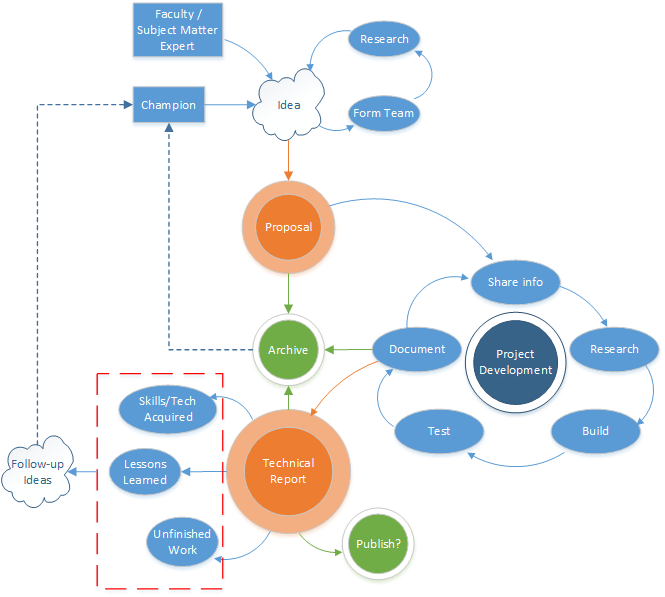
\includegraphics[width=\linewidth]{figs/project-life-cycle.png}
  %\caption{A PDD is the first piece of documentation to be archived in the project life cycle. Since the life cycle can be iterative, a new design document may also refer to one or more previous SPPs.}
%\label{fig:lifecycle}
%\end{figure}

% \section{Secondary Objectives}
% \label{sec:secondary-obj}
% Secondary Objectives are lower priority or bonus objectives that are significant but not the main focus of the project. This template does not have secondary objectives.

\section{Benefit to SPEX}
\label{sec:Benefit to SPEX}
% One of the core values of SPEX is to provide opportunities for academic and professional growth for its members,
% and to challenge them with interesting projects.
% In this section, explain how the project would benefit SPEX members as students,
% space enthusiasts, and young professionals.

SPEX's involvement in this globally-identified competition will serve to provide exposure and merit to the team and any sponsors involved in contributing.
Additionally, individual students engaged in this endeavor will also benefit by improving their technical knowledge and abilities while
participating in a major event which can also be used to improve their professional skillset.

% Below I have used subsections to identify key ideas in this section. These particular subsections are not required as part of the SPEX Standard, but serve as an example of using subsections in a text

\subsection{Benefit to RIT}
\label{subsec:Benefit to RIT}
By attending the event and competing against top universities, RIT will be able to use this as an opportunity to showcase
how passionate and involved their students are in space exploration. This involvement can be used in media as a tool for
achieving more funds and attracting new students to the University. Since RIT has not been involved with IREC before, SPEX's attendance at
this competition can also show how the University and its students are growing and taking on new challenges.

\subsection{Partnership with Launch Initiative}
\label{subsec:Partnership with Launch Initiative}
Since the founding of SPEX, there has never been a strong relationship with the Launch Initiative team. By cooperatively participating
in this event, a great opportunity is presented to create a good relationship between two of the largest space-related teams on
campus. In the future, united efforts between the two teams could result in more advanced projects which will provide
even more exposure to both RIT space teams.

\section{Implementation}
\label{sec:Implementation}

\subsection{Selection}
\label{subsec:Selection}
  % What path do you anticipate the project to take?
A decision matrix was created which accounts for the following factors and assigned a maximum possible
score based on importance to the selection process:
\begin{itemize}
  \item \textbf{Scientific Relevance (10 pts)}
  \begin{itemize}
    \item How does this payload contribute to the scientific community?
  \end{itemize}

  \item \textbf{Potential for Excellent Technical Execution (15 pts)}
  \begin{itemize}
    \item How feasible is it for the SPEX team to have great technical success with this endeavor?
  \end{itemize}

  \item \textbf{Time Required/ Complexity (5 pts)}
  \begin{itemize}
    \item Will this payload result in too much time being spent on research and development?
  \end{itemize}

  \item \textbf{Constructability (5 pts)}
  \begin{itemize}
    \item Does this payload require large amounts of machining and assembly or materials that are difficult to work with?
  \end{itemize}

  \item \textbf{Cost (5 pts)}
  \begin{itemize}
    \item How expensive will this be?
  \end{itemize}

  \item \textbf{Weight (5 pts)}
  \begin{itemize}
    \item Will it be easy to meet the 8.8lbs minimum requirement?
  \end{itemize}

  \item \textbf{Programmability (5 pts)}
  \begin{itemize}
    \item Does this payload require the use or creation of advanced software?
  \end{itemize}

  \item \textbf{"WOW" Factor (5 pts)}
  \begin{itemize}
    \item Is this payload attractive? Will it stick out among others?
  \end{itemize}
\end{itemize}

Based on the results of the individual scoring of each idea throughout the team, the "Hyperion" payload was selected to move forward with
an average score of 44 out of a maximum 55 points.

\subsection{Payload Details}
\label{subsec:Payload Details}
Hyperion is modeled after the black box technology found in aircraft. It represents a combination of two initially separate concepts of extreme self-diagnostics
and an airbag deployment mechanism for assisted landing similar to the Spirit and Opportunity Mars rovers. As per the IREC rules and requirements, the payload will
follow a traditional CubeSat standard. It is estimated that a 3U (10cm x 10cm x 30cm) volume will be utilized.

On the self-diagnostics side, data gathered from the rocket and the payload will be written to nonvolatile
memory as well as transmitted to a receiving ground station. The data gathered within the payload includes linear acceleration, angular rate, magnetic field detection,
temperature, absolute barometric pressure, GPS information, pressure within the landing balloons, and a variety of analog measurements from the circuit itself. Other data
gathered from the rocket includes vibration, mechanical strain, and a potential for engine data depending on the engine selected for use by LI.

During apogee at 10,000 feet, Hyperion will separate from the rocket and fall back to Earth with a controlled descent from a parachute. At a sufficient altitude, Hyperion will
electrically open valves that control the flow of CO2 from compressed canisters to inflate the balloons before striking the ground with a designed energy. These designed impact
conditions will allow for proof of concept without subjecting the payload to unnecessary stresses.

\subsection{Timeline}
\label{subsec:Timeline}
  % Be as detailed as you can, but it's okay if there are unknowns.
  % At the very least, specify how many semester you expect the project to take until it reaches completion.
The timeline is based largely around two important dates. The first is the hand-off of the external mechanical design to LI on November 1st which will provide time for LI
to incorporate Hyperion into their own designs. The second important date is the competition itself. Although the specific day has not been announced yet, past competition dates
suggest that it will be held during late June. The timeline is as follows:
\begin{itemize}
  \item September 1st: Begin narrowing down payload ideas using a decision matrix based on the SDL Payload Challenge scoring rubric
  \item September 8th: Decide on the specific payload and make a plan of action for research and design
  \item October 1st: Present a preliminary design with estimates for size, cost, and weight
  \item November 1st: Mechanical design delivery to LI. No changes to the external frame can be made after this point
  \item Semester's End: Final hardware design completed and materials ordered
  \item April 1st: Integration testing of rocket and payload
  \item April/May: Test launch of rocket and payload
  \item June 22nd-24th: Intercollegiate Rocket Engineering Competition
\end{itemize}

This timeline provides SPEX with roughly one month until a preliminary design is created. After this, there will be another month to refine
the design before the final size and interface details must be provided to LI. After this point, there will be more internal
design and development for the remainder of the semester with a goal of purchasing all materials by the semester's end.
If this timeline can be adhered to, then the entire spring semester and summer months leading up to the competition can be
used for manufacturing, programming, integration, testing, and characterization.

\subsection{Deliverables}
\label{subsec:Deliverables}
  % When all is said and done, what will you have to show for it?
  % Examples: Hardware, software, poster, ImagineRIT demo, presentations, technical papers...
In order to be compliant with the SDL Payload Challenge requirements, a poster is needed as part of the judging criteria.
Other deliverables for this project include the open-source technical documentation such as circuit schematics, CAD drawings,
and embedded software. The final deliverable is a functioning payload module conforming to the IREC SDL payload challenge
standard with accompanying ground station hardware and operating documentation.

\section{Externalities}
\label{subsec:Externalities}
  % Things not directly related to the work or outcomes, but related to the project as a whole.
\subsection{Prerequisite Skills}
\label{subsec:Prerequisite Skills}
  % Which skills do team members need to have before work can start (not including skills that will be learned ``on the job'')?
To participate in this endeavor, there are no prerequisite skills. However, for the project to succeed, there will need to be
individuals who are proficient in computer-aided design and mechanical analysis for the structure of the payload. These members
are responsible for the selection of materials and the construction of the frame, airbag deployment, and the return parachute.
There will also need to be individuals proficient in electronic design, specifically with respect to printed circuit boards.
These members are responsible for sensor selection and implementation, power regulation, and maintaining electrical connections
between each part of the payload. Individuals proficient in programming will be required for embedded systems design, ground-station processing,
and the overarching communication network that is needed to meet the goals of the project.  Finally, there will need to be some individuals
who are willing to fill the role of system engineers who will be responsible for communicating with the separate LI team and acting as a resource
to those designing the hardware and software.

\subsection{Funding Requirements}
\label{subsec:Funding Requirements}
  % Estimate costs that would be needed to meet objectives.
Although the preliminary design has not yet been completed, component selection has already begun and estimates for total cost have been
gathered. The high-level cost breakdown assessment is as follows:
\begin{itemize}
  \item \textbf{Mechanical Construction - \$950}
  \begin{itemize}
    \item Aluminum - 200
    \item Kevlar - 60
    \item Nomex - 90
    \item CO2 Canisters - 40
    \item Solenoids - 300
    \item Fittings - 80
    \item Rocket Connectors - 150
    \item Miscellaneous - 30
  \end{itemize}

  \item \textbf{Electrical - \$320}
  \begin{itemize}
    \item Sensors - 220
    \item PCBs - 40
    \item Other Components - 60
  \end{itemize}

  \item \textbf{Communications - \$180}
  \begin{itemize}
    \item Radios - 100
    \item Antennas - 80
  \end{itemize}

  \item \textbf{Total - \$1450}
\end{itemize}

Although these numbers are preliminary, a realistic estimate of total cost with an included margin is roughly 1,700 dollars. The SPEX internal budget has allocated 500 dollars
towards this project. The remaining funds need to come from external sources. One such potential source is the Students for the Exploration and Development
of Space (SEDS) non-profit which has grants available for participating chapters. If additional sources are needed, the preliminary designs and this
project definition document will be used in a fundraising campaign to reach out to local individuals and businesses.

\subsection{Faculty Support}
\label{subsec:Faculty Support}
  % Identify faculty that will be involved (or would need to be involved) to meet objectives.
  % Note that if a professor is the Principal Investigator (P.I.) for a project, there still needs to be a student as the SPEX Project Champion.
SPEX members will consistently seek faculty support throughout the design process. Although no faculty have yet been willing to dedicate a
large block of time to assist this project. There have been multiple offers to provide guidance in a limited capacity. Although this project can succeed solely
with SPEX members, this is a great opportunity to cooperate with RIT professors and researchers who can provide their knowledge and experience.

\subsection{Long-Term Vision}
\label{sec:Long-Term Vision}
The long-term goal of this project is to establish a relationship between LI and SPEX in which the teams can continue to cooperate
in future IRECs and other multi-team projects. By working off of past successes, SPEX and LI can grow together and eventually compete in the
advanced category against the leading schools. Competing in this event will not only achieve SPEX's mission of giving students the opportunity to gain hands-on
experience working with space systems, but will also facilitate an evolution into a team that is involved in competitive space-systems engineering.

\section*{Acknowledgements}
\label{subsec:Acknoledgements}
The author would like to thank all of SPEX's sponsors and supporters. The author would also like to thank those who reviewed this document and provided feedback
as well as SPEX alumni Phil Linden for providing a great template for writing documents such as these.
\onecolumn
\appendices{}

\end{document}
